\documentclass[12pt,a4paper]{article}
\usepackage[utf8]{inputenc}
\usepackage[spanish,es-tabla]{babel}
\usepackage{geometry}
\usepackage{graphicx}
\usepackage{multirow}
\usepackage{tabularx}
\usepackage{mathptmx}
\usepackage{fancyhdr}
\usepackage{array}
\usepackage[table]{xcolor}
\usepackage{titlesec}
\usepackage{setspace}
\usepackage{microtype}
\usepackage{lastpage}
\usepackage{booktabs}
\usepackage{enumitem}
\usepackage{amsmath}
\usepackage{amsfonts}
\usepackage{amssymb}

\graphicspath{{images/}{../images/}{./}}

\geometry{
    top=4.7cm,
    bottom=2.5cm,
    left=2.5cm,
    right=2.5cm,
    headheight=3.9cm,
    headsep=0.4cm
}

\setstretch{1.15}
\setlength{\parindent}{0pt}
\setlength{\parskip}{0.45em}
\setlength{\tabcolsep}{4pt}

\titleformat{\section}
  {\normalfont\fontsize{12}{14.5}\bfseries}{\thesection.}{0.6em}{\uppercase}
\titlespacing*{\section}
  {0pt}{1.8ex plus 0.4ex minus 0.2ex}{0.6ex plus 0.2ex}

\titleformat{\subsection}
  {\normalfont\fontsize{11.5}{13.5}\bfseries}{\thesubsection.}{0.5em}{}
\titlespacing*{\subsection}
  {0pt}{1.4ex plus 0.3ex minus 0.1ex}{0.4ex plus 0.1ex}

\titleformat{\subsubsection}
  {\normalfont\fontsize{10.5}{12.5}\bfseries\itshape}{\thesubsubsection.}{0.4em}{}
\titlespacing*{\subsubsection}
  {0pt}{1.1ex plus 0.2ex minus 0.1ex}{0.3ex plus 0.1ex}

\newcolumntype{Y}{>{\centering\arraybackslash}X}
\newcolumntype{L}{>{\raggedright\arraybackslash}X}
\newcolumntype{C}{>{\centering\arraybackslash}X}

\definecolor{headerred}{RGB}{180, 0, 0}
\definecolor{darkred}{RGB}{140, 0, 0}
\definecolor{lightgraybg}{RGB}{248, 248, 248}
\definecolor{tableheader}{RGB}{232, 238, 246}

\newcommand{\docCodigo}{TI-SIGE-ENT-S1-002}
\newcommand{\docVersion}{1.0}
\newcommand{\docProceso}{INGENIERÍA DE REQUERIMIENTOS / GOBERNANZA}
\newcommand{\docElaboracion}{18/08/2026}
\newcommand{\docRevision}{PENDIENTE DE REVISIÓN}
\newcommand{\docTitulo}{IDENTIFICACIÓN DE ACTORES, MATRIZ DE PODER/INTERÉS Y MATRIZ RACI}
\newcommand{\docOrganizacion}{FACULTAD DE INGENIERÍA EN SISTEMAS, ELECTRÓNICA E INDUSTRIAL}
\newcommand{\docSubOrganizacion}{CARRERA DE INGENIERÍA DE SOFTWARE}

\newcommand{\encabezadofrecuente}{%
    \renewcommand{\arraystretch}{1.15}%
    \noindent\makebox[\textwidth][c]{%
    \begin{tabularx}{\textwidth}{|>{\centering\arraybackslash}m{2.8cm}|Y|>{\centering\arraybackslash}m{4.8cm}|}
        \hline
        \multirow{4}{2.8cm}{\centering\raisebox{-1.15cm}{
\includegraphics[width=2.5cm,height=2.0cm,keepaspectratio]{images/logo.png}}}
        & \textbf{\fontsize{9}{11}\selectfont \docOrganizacion} 
        & \textbf{\fontsize{8}{10}\selectfont CÓDIGO:} \fontsize{8}{10}\selectfont \docCodigo \\
        \cline{3-3}
        & \textbf{\fontsize{8.5}{10.5}\selectfont \docSubOrganizacion} 
        & \textbf{\fontsize{8}{10}\selectfont VERSIÓN:} \fontsize{8}{10}\selectfont \docVersion \\
        \cline{2-3}
        & \textbf{\fontsize{8}{10}\selectfont PROCESO:} \fontsize{8}{10}\selectfont \docProceso 
        & \textbf{\fontsize{8}{10}\selectfont ELABORACIÓN:} \fontsize{8}{10}\selectfont \docElaboracion \\
        \cline{2-3}
        & \textbf{\fontsize{8.5}{10.5}\selectfont \docTitulo} 
        & \textbf{\fontsize{8}{10}\selectfont ÚLTIMA REVISIÓN:} \fontsize{8}{10}\selectfont \textbf{\textcolor{darkred}{\docRevision}} \\
        \hline
    \end{tabularx}%
    }%
}

\pagestyle{fancy}
\fancyhf{}
\fancyhead[C]{\encabezadofrecuente}
\fancyfoot[C]{\fontsize{10}{12}\selectfont Página \thepage\ de \pageref{LastPage}}
\renewcommand{\headrulewidth}{0pt}

\begin{document}

\section{Título}
\textbf{Denominación del Entregable:} Identificación de Actores, Matriz de Poder/Interés y Matriz RACI -- Código EDT: 1.2



\section{Introducción}
La identificación rigurosa de los interesados (\textit{Stakeholders}) y la definición de sus niveles de autoridad y responsabilidad constituyen un factor determinante para el éxito de la plataforma \textbf{SIGE}. En este documento se formalizan los actores institucionales que intervienen en el flujo documental del SGC de la FISEI, su categorización mediante la Matriz de Poder/Interés y la asignación de responsabilidades operativas a través de una Matriz RACI.

\section{Objetivo}

\subsection{Objetivo General}
Identificar, caracterizar y mapear la totalidad de actores institucionales y procesos del Sistema de Gestión de Calidad (SGC) en la FISEI UTA mediante matrices de Poder/Interés y RACI para delimitar el control de acceso por roles (RBAC) en el sistema SIGE.

\subsection{Objetivos Específicos}
\begin{itemize}[leftmargin=1.5em, itemsep=1.5pt]
    \item Caracterizar los 5 roles del sistema (Docente Elaborador, Coordinador de Área, Coordinador de Carrera, Subdecano y Administrador SGC).
    \item Construir la Matriz de Poder vs. Interés para determinar las estrategias de comunicación y gestión de expectativas.
    \item Estructurar la Matriz RACI para los 10 procesos críticos de elaboración, revisión, aprobación y auditoría.
\end{itemize}

\section{Alcance}

\subsection{Límites de la Caracterización (In-Scope)}
\begin{itemize}[leftmargin=1.5em, itemsep=1.5pt]
    \item Actores de la estructura académica y de gestión de calidad de la FISEI.
    \item Procesos de aprobación jerárquica en cascada para planes de trabajo e informes de cumplimiento.
\end{itemize}

\subsection{Exclusiones (Out-of-Scope)}
\begin{itemize}[leftmargin=1.5em, itemsep=1.5pt]
    \item Personal administrativo de nómina central de la universidad o departamentos externos de compras públicas.
\end{itemize}

\section{Definiciones}
\begin{itemize}[leftmargin=1.5em, itemsep=2pt]
    \item \textbf{RACI:} Modelo de asignación de responsabilidades: \textit{Responsible} (R), \textit{Accountable} (A), \textit{Consulted} (C), \textit{Informed} (I).
    \item \textbf{RBAC (\textit{Role-Based Access Control}):} Mecanismo de seguridad que restringe el acceso a recursos según el rol asignado al usuario.
    \item \textbf{Poder / Interés:} Herramienta de gestión de stakeholders que clasifica a los interesados según su nivel de autoridad e impacto en el proyecto.
    \item \textbf{Cascada de Firmas:} Secuencia jerárquica obligatoria de legalización electrónica.
\end{itemize}

\section{Responsabilidades}
\begin{itemize}[leftmargin=1.5em, itemsep=2pt]
    \item \textbf{Líder de Proyecto / Arquitecto (Steeven Toala):} Diseño de la matriz RACI, modelo de gobernanza y especificación de roles RBAC.
    \item \textbf{Analista de Requerimientos (Heidy Villavicencio):} Mapeo de interesados, entrevistas de caracterización y matriz de poder/interés.
    \item \textbf{Docente Tutor (Ing. Paulo Torres):} Validación y aprobación del esquema de gobernanza y niveles de firma.
\end{itemize}

\section{Normativa Legal y Técnica}
\begin{itemize}[leftmargin=1.5em, itemsep=2pt]
    \item \textbf{Estatuto Orgánico de la Universidad Técnica de Ambato:} Atribuciones de directores de departamento, coordinadores y docentes.
    \item \textbf{Guía del PMBOK (7ma Edición):} Dominio de Desempeño de los Interesados.
    \item \textbf{Estándar ISO/IEC 27001:2022:} Control de acceso y segregación de funciones en sistemas de información.
\end{itemize}

\section{Método, Políticas y Contenidos}
Se aplicó la metodología de mapeo de interesados basada en entrevistas a directivos y análisis documental de la estructura orgánica de la FISEI:

\begin{figure}[htbp]
    \centering
    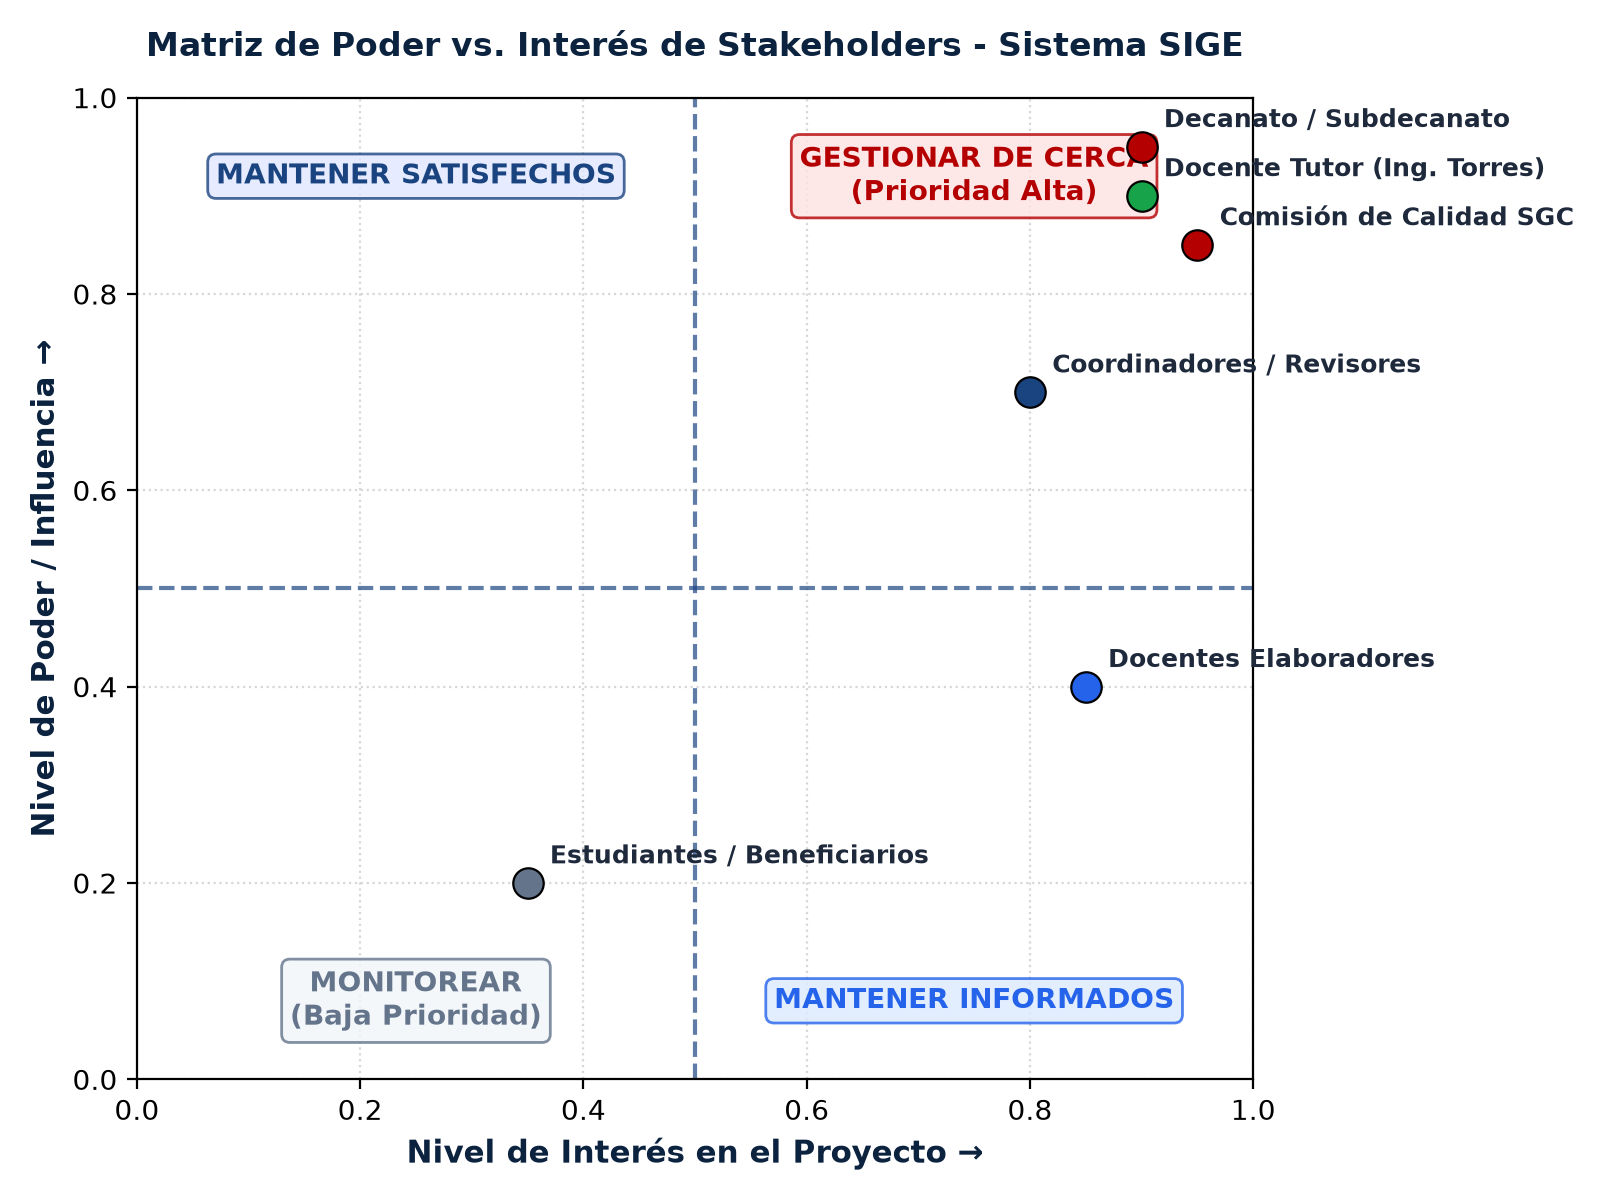
\includegraphics[width=0.82\textwidth,height=5.5cm,keepaspectratio]{images/s1_02_quadrant_chart.png}
    \caption{Matriz de Poder vs. Interés de los Interesados del Sistema SIGE.}
    \label{fig:s1_02_poder_interes}
\end{figure}

\section{Descripción de actividades}

\subsection{Caracterización Detallada de Actores y Roles}

\begin{table}[htbp]
\centering
\small
\renewcommand{\arraystretch}{1.2}
\begin{tabularx}{\textwidth}{|>{\bfseries}m{3.2cm}|m{3.2cm}|X|}
\hline
\rowcolor{tableheader}
Rol en SIGE & Cargo Institucional & Responsabilidad Principal en el Flujo Documental \\
\hline
\textbf{Docente Elaborador} & Docente Titular / Ocasional & Elabora el Plan de Trabajo (P7-T1) y el Informe de Cumplimiento (P7-T2), carga evidencias en MinIO y estampa la Firma 1. \\
\hline
\textbf{Coordinador de Área} & Docente Coordinador de Área & Revisa pertinencia de actividades de la matriz, audita evidencias, emite observaciones y estampa la Firma 2. \\
\hline
\textbf{Coordinador de Carrera} & Director / Coordinador Carrera & Verifica articulación curricular, aprueba la planificación y rendición de cuentas, y estampa la Firma 3. \\
\hline
\textbf{Validador / Subdecano} & Subdecano FISEI / Consejo & Valida y legaliza los expedientes consolidados para fines de acreditación institucional. \\
\hline
\textbf{Administrador SGC} & Administrador del Sistema & Parametriza catálogos, gestiona usuarios y autoriza prórrogas/habilitaciones extemporáneas con justificación. \\
\hline
\end{tabularx}
\caption{Caracterización de Actores y Roles del Sistema SIGE.}
\label{tab:actores_roles}
\end{table}

\subsection{Matriz de Asignación de Responsabilidades (RACI)}

\begin{table}[htbp]
\centering
\small
\renewcommand{\arraystretch}{1.15}
\begin{tabularx}{\textwidth}{|X|>{\centering\arraybackslash}m{1.5cm}|>{\centering\arraybackslash}m{1.5cm}|>{\centering\arraybackslash}m{1.5cm}|>{\centering\arraybackslash}m{1.5cm}|>{\centering\arraybackslash}m{1.5cm}|}
\hline
\rowcolor{tableheader}
Proceso Documental del SGC & Docente Elaborador & Coord. Área & Coord. Carrera & Subdecano Consejo & Admin SGC \\
\hline
1. Definición de Catálogo de Actividades & I & C & C & I & \textbf{A / R} \\
\hline
2. Creación del Plan de Trabajo (P7-T1) & \textbf{A / R} & C & I & I & I \\
\hline
3. Revisión de Matriz de Planificación & R & \textbf{A / R} & C & I & I \\
\hline
4. Cascada de Firmas Inicial (P7-T1) & \textbf{R (F1)} & \textbf{R (F2)} & \textbf{A / R (F3)} & I & I \\
\hline
5. Carga de Evidencias en MinIO S3 & \textbf{A / R} & I & I & I & I \\
\hline
6. Seguimiento y Control de Matrices & R & \textbf{A / R} & I & I & I \\
\hline
7. Habilitación de Prórroga Extemporánea & I & C & C & I & \textbf{A / R} \\
\hline
8. Elaboración del Informe (P7-T2) & \textbf{A / R} & I & I & I & I \\
\hline
9. Dictamen y Observaciones por Párrafo & R & \textbf{A / R} & C & I & I \\
\hline
10. Legalización Final del Expediente & I & I & R & \textbf{A / R} & I \\
\hline
\end{tabularx}
\caption{Matriz RACI de Procesos de Gestión Documental SGC.}
\label{tab:matriz_raci}
\end{table}

\vspace{0.3cm}

% =============================================================
% 10. FIRMAS DE RESPONSABILIDAD
% =============================================================
\section{Firmas de Responsabilidad}

\noindent
\renewcommand{\arraystretch}{1.2}
\begin{tabularx}{\textwidth}{|>{\raggedright\arraybackslash}m{2.9cm}|>{\raggedright\arraybackslash}X|>{\centering\arraybackslash}m{4.6cm}|>{\centering\arraybackslash}m{2.3cm}|}
    \hline
    \rowcolor{headerred}
    \textcolor{white}{\textbf{ACCIÓN}} & \textcolor{white}{\textbf{NOMBRE Y CARGO}} & \textcolor{white}{\textbf{FIRMA}} & \textcolor{white}{\textbf{FECHA}} \\
    \hline
    \textbf{Elaborado por:} & Steeven Toala\newline \textit{Líder de Proyecto / Arquitecto Software} & \parbox[c]{4.4cm}{\centering\vspace{4pt}
\includegraphics[height=1.5cm,width=4.0cm,keepaspectratio]{images/firma_steveen.png}\vspace{4pt}} & 18/08/2026 \\
    \hline
    \textbf{Revisado por:} & Heidy Villavicencio\newline \textit{Analista de Requerimientos / UI-UX} & \parbox[c]{4.4cm}{\centering\vspace{4pt}
\includegraphics[height=1.5cm,width=4.0cm,keepaspectratio]{images/firma_heidi.png}\vspace{4pt}} & 18/08/2026 \\
    \hline
    \textbf{Aprobado por:} & Ing. Paulo Torres\newline \textit{Docente Tutor - Gestión Proyectos Software} & \parbox[c]{4.4cm}{\centering\vspace{10pt}\textbf{\textcolor{gray!80}{\scriptsize [ PENDIENTE DE APROBACIÓN ]}}\vspace{10pt}} & \textbf{\textcolor{gray!90}{Pendiente}} \\
    \hline
\end{tabularx}

\vspace{0.4cm}

% =============================================================
% 11. CONTROL DE CAMBIOS
% =============================================================
\section{Control de Cambios}

\noindent
\renewcommand{\arraystretch}{1.2}
\begin{tabularx}{\textwidth}{|>{\hsize=0.45\hsize\centering\arraybackslash}X|>{\hsize=1.55\hsize\raggedright\arraybackslash}X|>{\hsize=1.2\hsize\raggedright\arraybackslash}X|>{\hsize=0.8\hsize\centering\arraybackslash}X|}
    \hline
    \rowcolor{gray!20}
    \textbf{Versión} & \textbf{Descripción del cambio} & \textbf{Responsable del cambio} & \textbf{Fecha de aprobación} \\
    \hline
    1.0 & Identificación formal de actores institucionales, matriz de poder/interés y matriz RACI & Steeven Toala / Heidy Villavicencio & \textbf{\textcolor{gray!90}{Pendiente de Revisión}} \\
    \hline
\end{tabularx}

\vspace{0.4cm}

% =============================================================
% 12. ANEXOS
% =============================================================
\section{Anexos}
\subsection*{Anexo 1: Organigrama Operativo de la FISEI UTA}
Estructura de dependencias entre Decanato, Subdecanato, Coordinaciones de Carrera, Coordinaciones de Área de Conocimiento y Cuerpo Docente.

\end{document}
